
% This LaTeX was auto-generated from MATLAB code.
% To make changes, update the MATLAB code and republish this document.

\documentclass{article}
\usepackage{graphicx}
\usepackage{color}

\sloppy
\definecolor{lightgray}{gray}{0.5}
\setlength{\parindent}{0pt}

\begin{document}

    
    
\subsection*{Contents}

\begin{itemize}
\setlength{\itemsep}{-1ex}
   \item Load and Preprocess Data
\end{itemize}
\begin{verbatim}
% Avita Sharma 5/1/2017
% Regression on Data from the US Census

% First run build_data.py
\end{verbatim}


\subsection*{Load and Preprocess Data}

\begin{verbatim}
clear, clc, close all

% load Panel Data
Panel = readtable('dataset.csv');
Panel.GDP = log(Panel.GDP);
Panel.uni = log(Panel.uni);
Panel.minw = log(Panel.minw);
Panel.eind = log(Panel.eind);
Panel.ecom = log(Panel.ecom);
% perform a Multilevel Mixed-Effects Modeling usin
% Ordinary Least Squares
lm_ols = fitlm(Panel, ['job ~ time + state +(time:state) + unemp + edu'...
                        '+ uni + minw + GDP + eind + ecom'])
lme_ols = fitlme(Panel, ['job ~ time + state +(time:state) + unemp + edu'...
                        '+ uni + minw + GDP + eind + ecom'])
figure();
plotResiduals(lm_ols,'fitted')
figure();
plotResiduals(lme_ols,'fitted')
\end{verbatim}

        \color{lightgray} \begin{verbatim}
lm_ols = 


Linear regression model:
    job ~ 1 + edu + uni + minw + GDP + eind + ecom + unemp + state*time

Estimated Coefficients:
                    Estimate         SE         tStat       pValue  
                   ___________    _________    ________    _________

    (Intercept)         5147.7       1716.4      2.9992    0.0029872
    state               1.0796       3.8741     0.27867      0.78074
    time               -2.9417      0.97875     -3.0056    0.0029272
    edu             0.00050057    0.0096209    0.052029      0.95855
    uni                -0.0208     0.044465    -0.46779      0.64035
    minw               0.38123      0.80697     0.47242      0.63705
    GDP                 80.066       26.186      3.0576    0.0024794
    eind              -0.29481       0.1486      -1.984     0.048382
    ecom              -0.22117      0.15184     -1.4566      0.14651
    unemp             0.050963     0.031541      1.6158      0.10743
    state:time     -0.00053973    0.0019255    -0.28031      0.77948


Number of observations: 255, Error degrees of freedom: 244
Root Mean Squared Error: 0.681
R-squared: 0.105,  Adjusted R-Squared 0.0687
F-statistic vs. constant model: 2.87, p-value = 0.0021

lme_ols = 


Linear mixed-effects model fit by ML

Model information:
    Number of observations             255
    Fixed effects coefficients          11
    Random effects coefficients          0
    Covariance parameters                1

Formula:
    job ~ 1 + edu + uni + minw + GDP + eind + ecom + unemp + state*time

Model fit statistics:
    AIC       BIC       LogLikelihood    Deviance
    540.27    582.77    -258.14          516.27  

Fixed effects coefficients (95% CIs):
    Name                 Estimate       SE           tStat       DF 
    '(Intercept)'             5147.7       1678.9      3.0661    244
    'state'                   1.0796       3.7896     0.28488    244
    'time'                   -2.9417      0.95741     -3.0726    244
    'edu'                 0.00050057    0.0094111     0.05319    244
    'uni'                    -0.0208     0.043496    -0.47822    244
    'minw'                   0.38123      0.78938     0.48295    244
    'GDP'                     80.066       25.615      3.1258    244
    'eind'                  -0.29481      0.14536     -2.0282    244
    'ecom'                  -0.22117      0.14853     -1.4891    244
    'unemp'                 0.050963     0.030853      1.6518    244
    'state:time'         -0.00053973    0.0018835    -0.28656    244


    pValue       Lower         Upper     
    0.0024132        1840.7        8454.8
      0.77598       -6.3849         8.544
    0.0023628       -4.8276       -1.0559
      0.95762     -0.018037      0.019038
      0.63292      -0.10648      0.064875
      0.62957       -1.1736        1.9361
    0.0019881        29.612        130.52
     0.043628      -0.58113    -0.0084958
      0.13776      -0.51373      0.071392
     0.099862    -0.0098092       0.11174
      0.77469    -0.0042497     0.0031702

Random effects covariance parameters (95% CIs):
Group: Error
    Name             Estimate    Lower      Upper  
    'Res Std'        0.66588     0.61053    0.72626

\end{verbatim} \color{black}
    
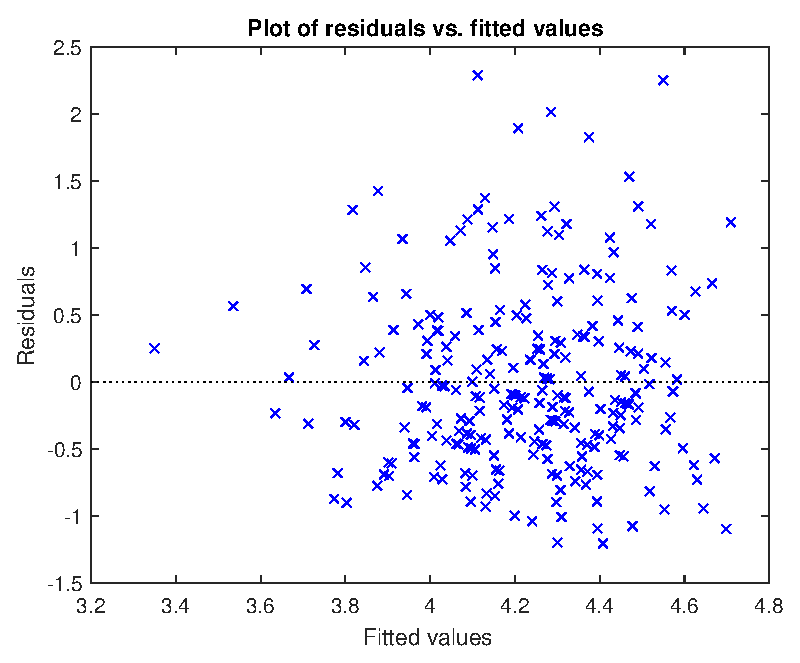
\includegraphics [width=4in]{regression_01.eps}

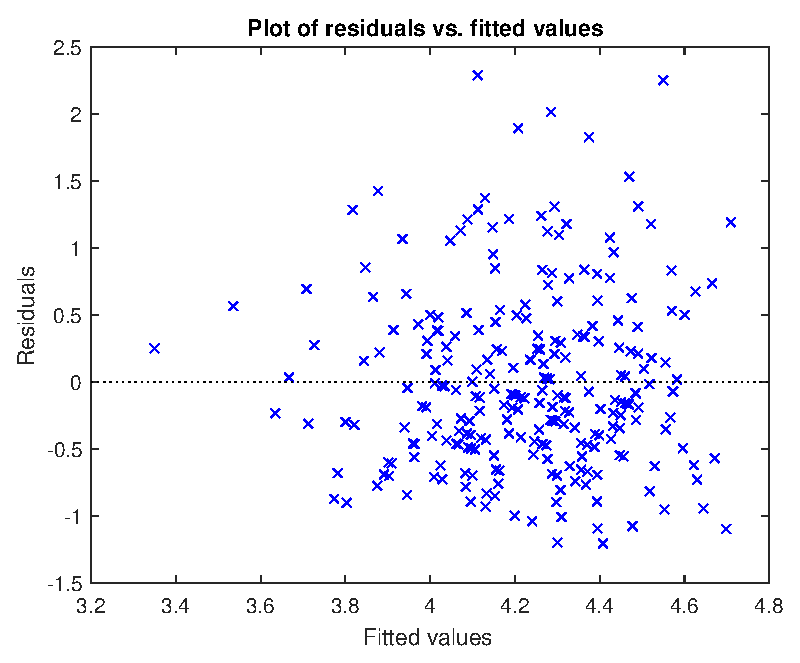
\includegraphics [width=4in]{regression_02.eps}



\end{document}
    
